\section{Review of Stationary and Non-stationary Kernels}
Based on Bochner's theorem, the Fourier transfor of a continious shift-invariant positive definite kernel $K(x,x')$ is a proper probability distribution function $\pi(\omega)$, assuming that $K(x,x')$ is properly scaled, that is
\begin{equation}
K(x,x') = \int \pi(\omega) e^{ i \omega^T (x - x') }\ d\omega = \mathbb{E}_{\omega}\big[ \phi_\omega (x) \phi_\omega (x')^* \big] 
\end{equation}
for $\phi_\omega (x)  =e^{j \omega^T x} = r \big( \cos (\omega x ) + i \sin (\omega x )\big)$. The density of $\omega$ is denoted by spectral density. 


TODO: produce some plots about the kernel choice for IMFS, plots like from the Turners presentation - elipsoids, a priori generated sample, a posteriori distribution given a few points


\begin{figure}[H]
\centering
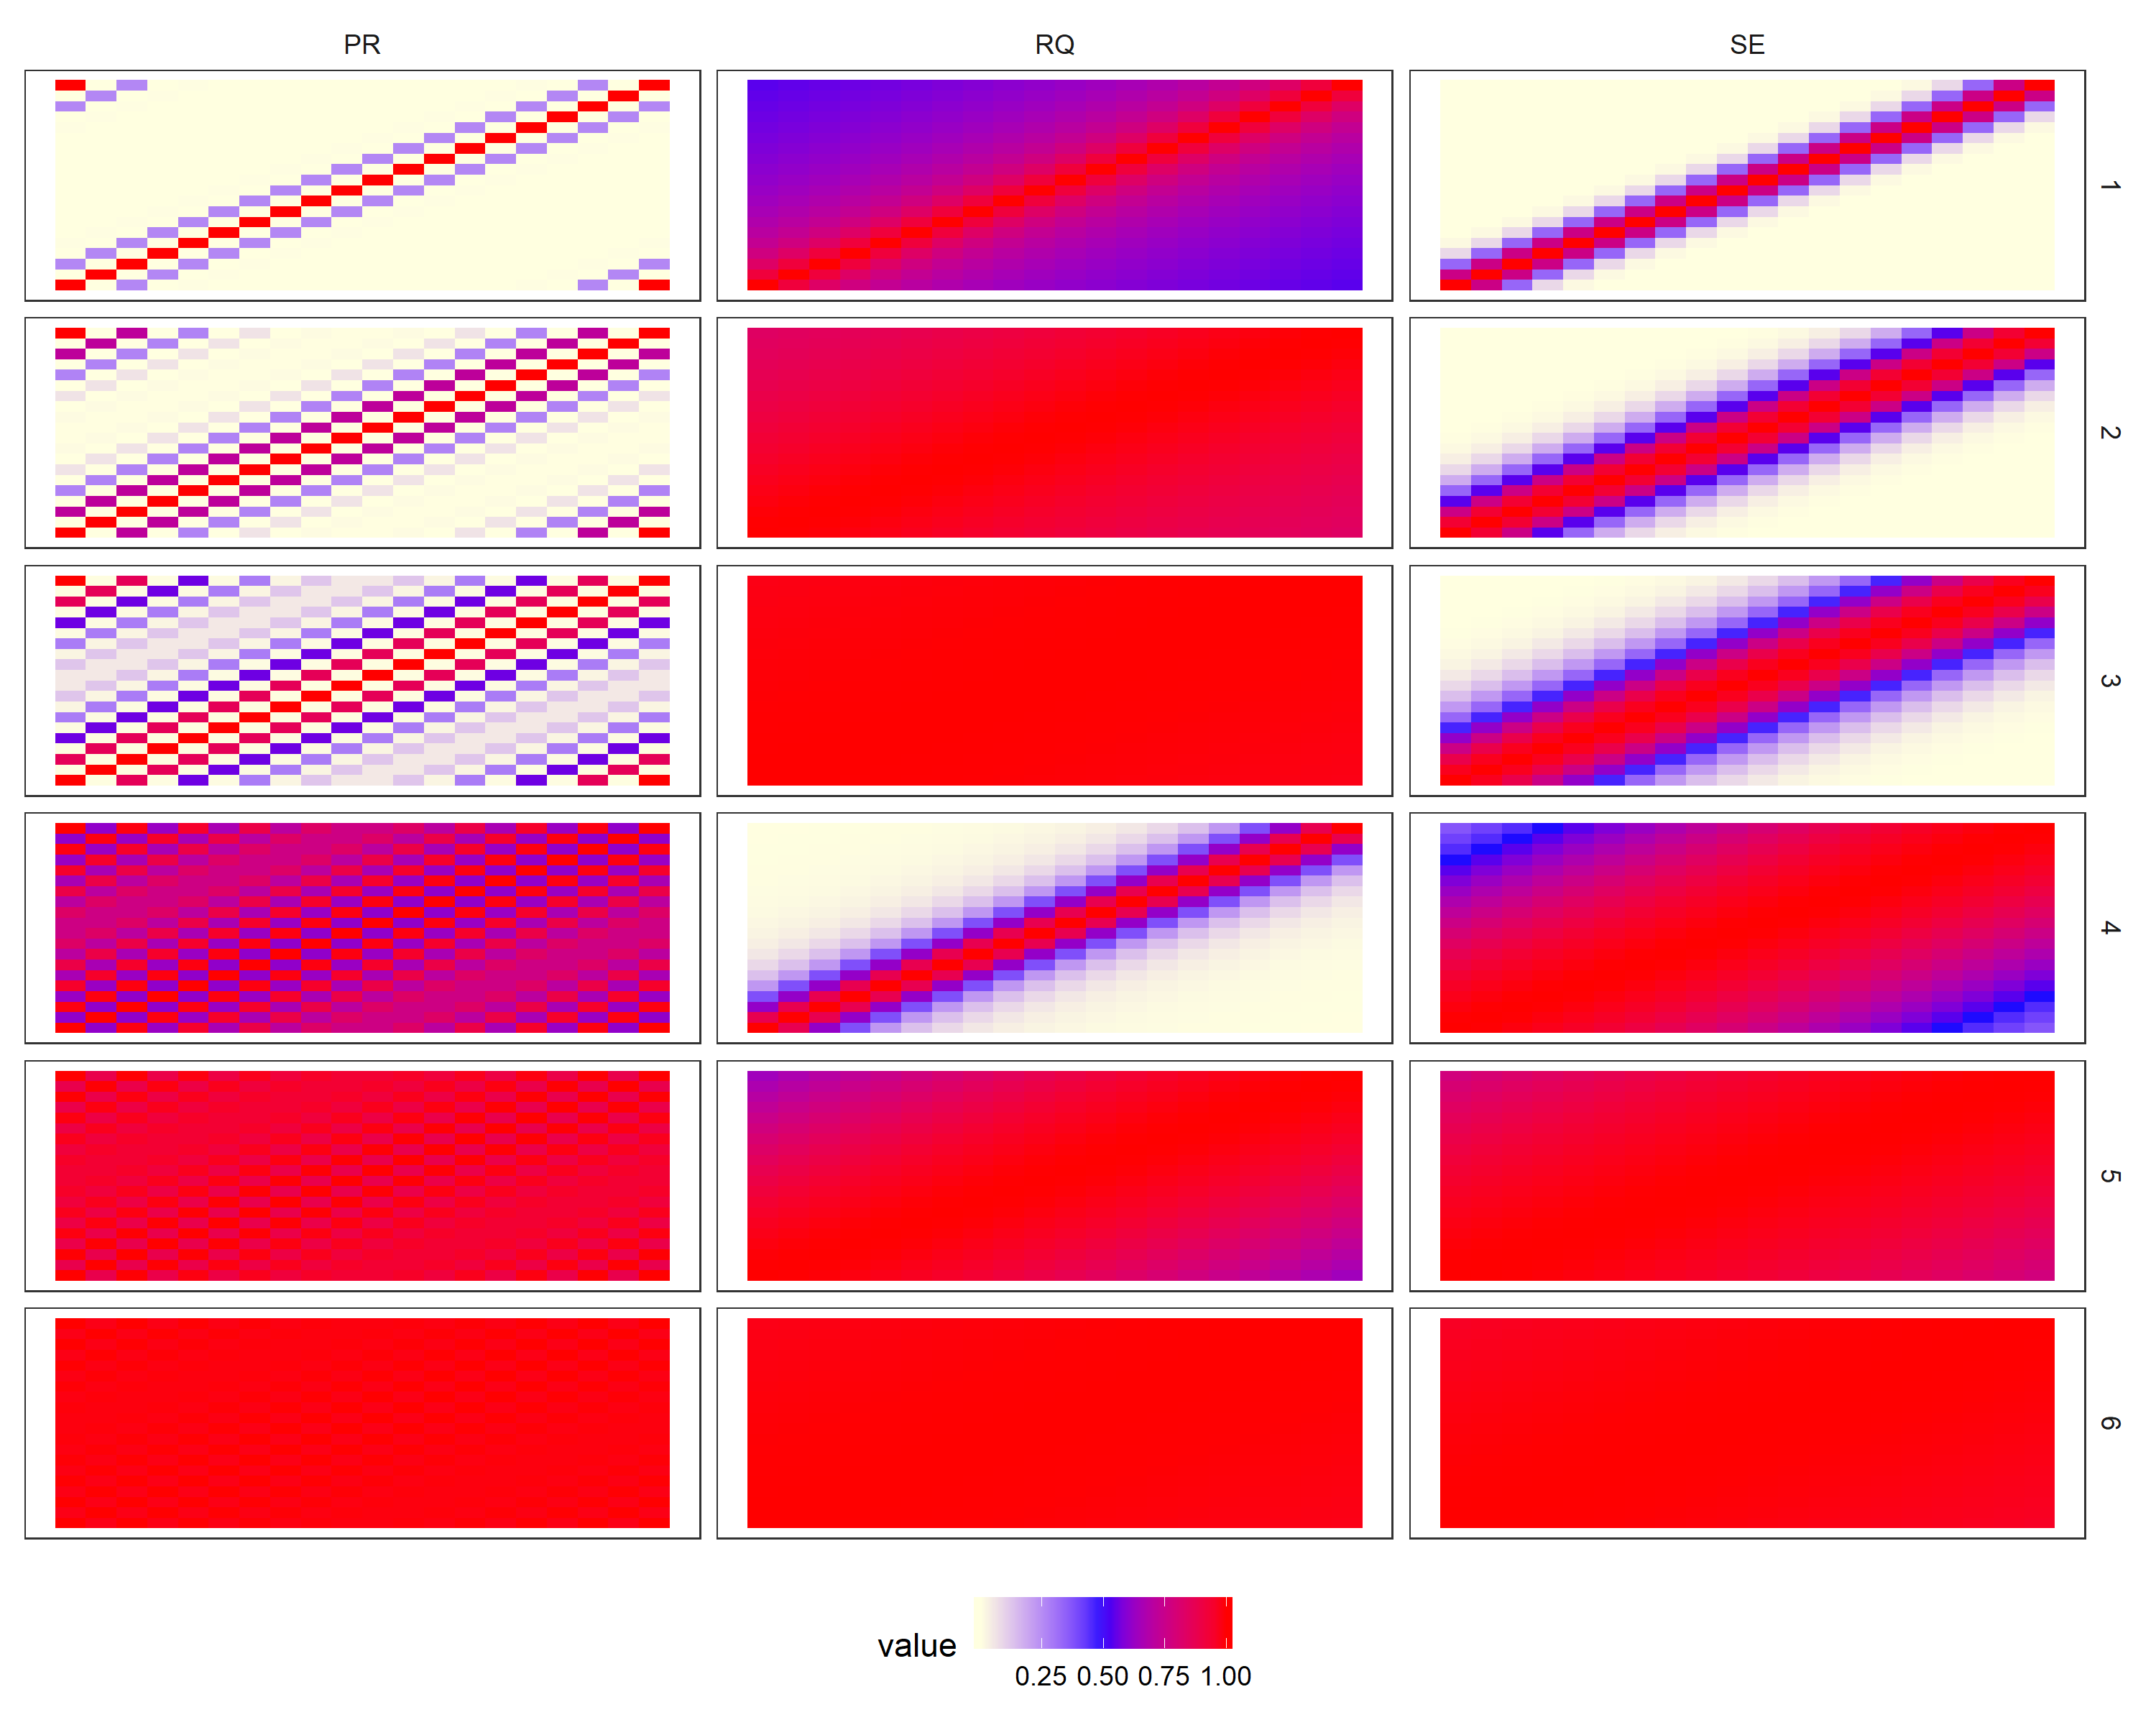
\includegraphics[scale = 0.15]{GP_illustrations/kernel_stationary.png}
\caption{Stationary kernels under 6 different sets of hyper-parameters.}\label{fig:}
\end{figure}

\begin{figure}[H]
\centering
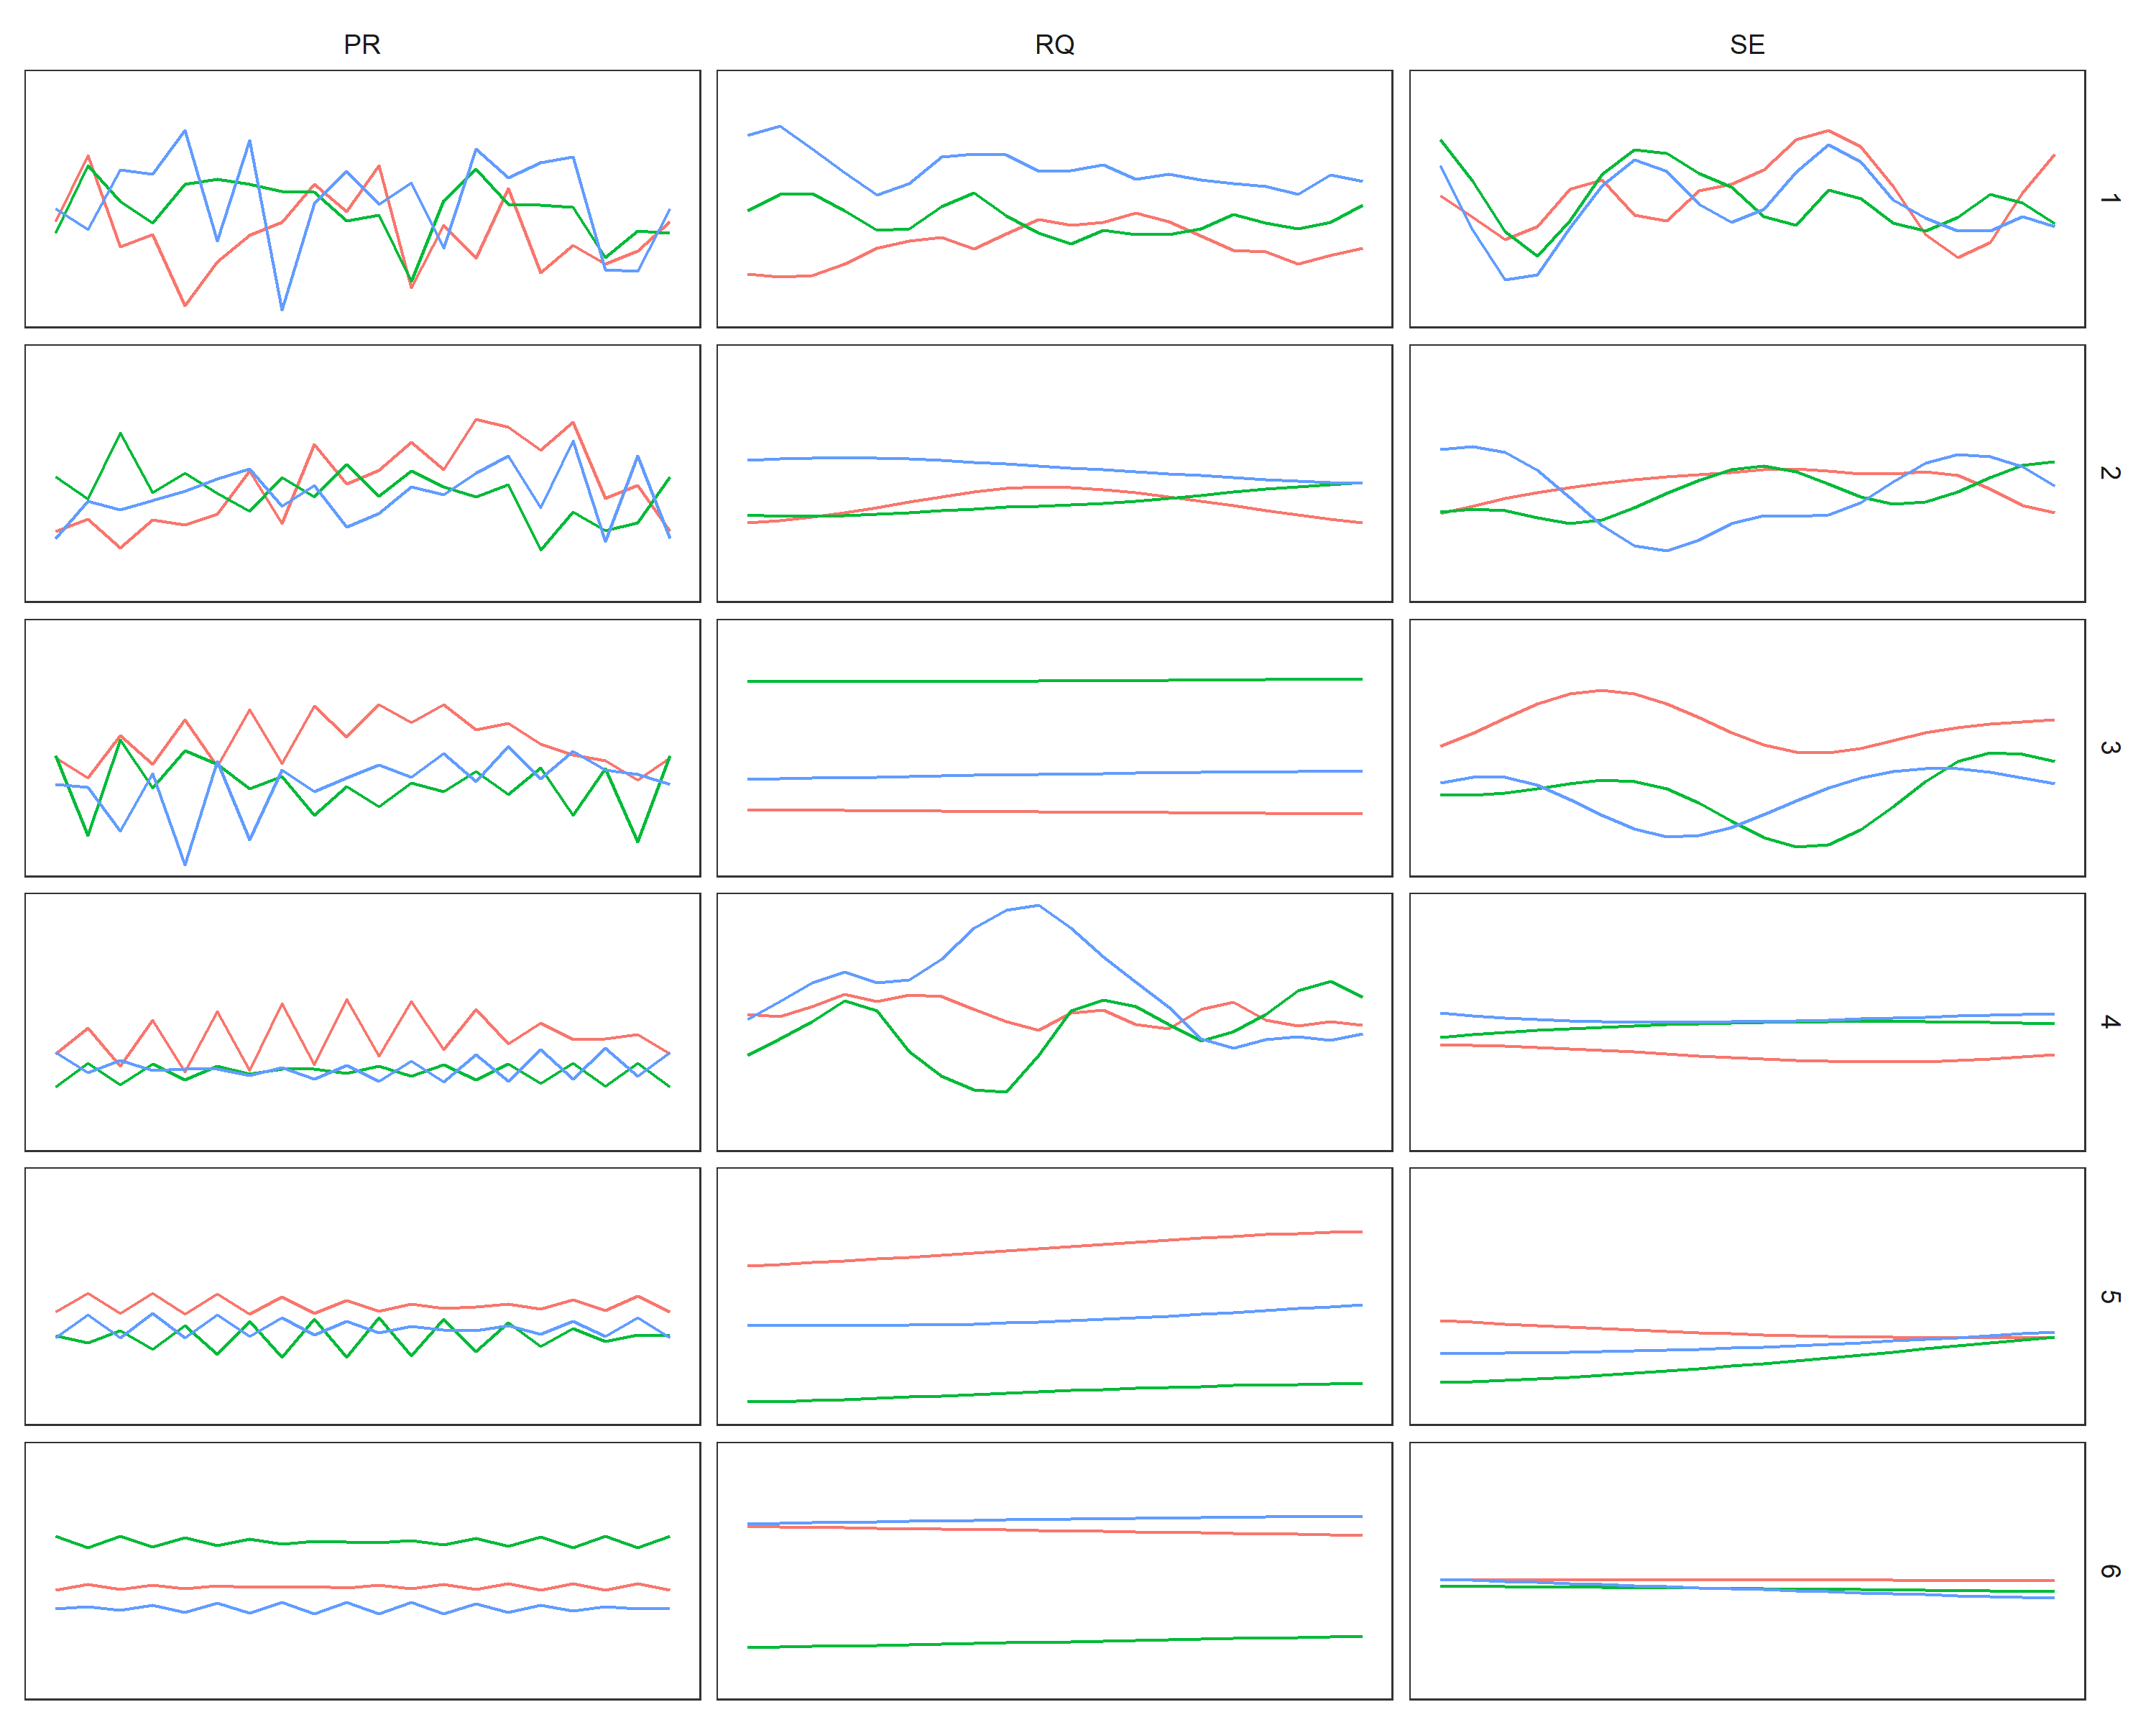
\includegraphics[scale = 0.15]{GP_illustrations/y_sim_stationary.png}
\caption{The 3 path of the signal $c_k$ simulated from the a priori distribution in Equation \eqref{eq:model_IMF_GP_k} under different stationary kernel assumptions (columns wise) and for 6 different sets of hyper-parameters.}\label{fig:}
\end{figure}

\begin{figure}[H]
\centering
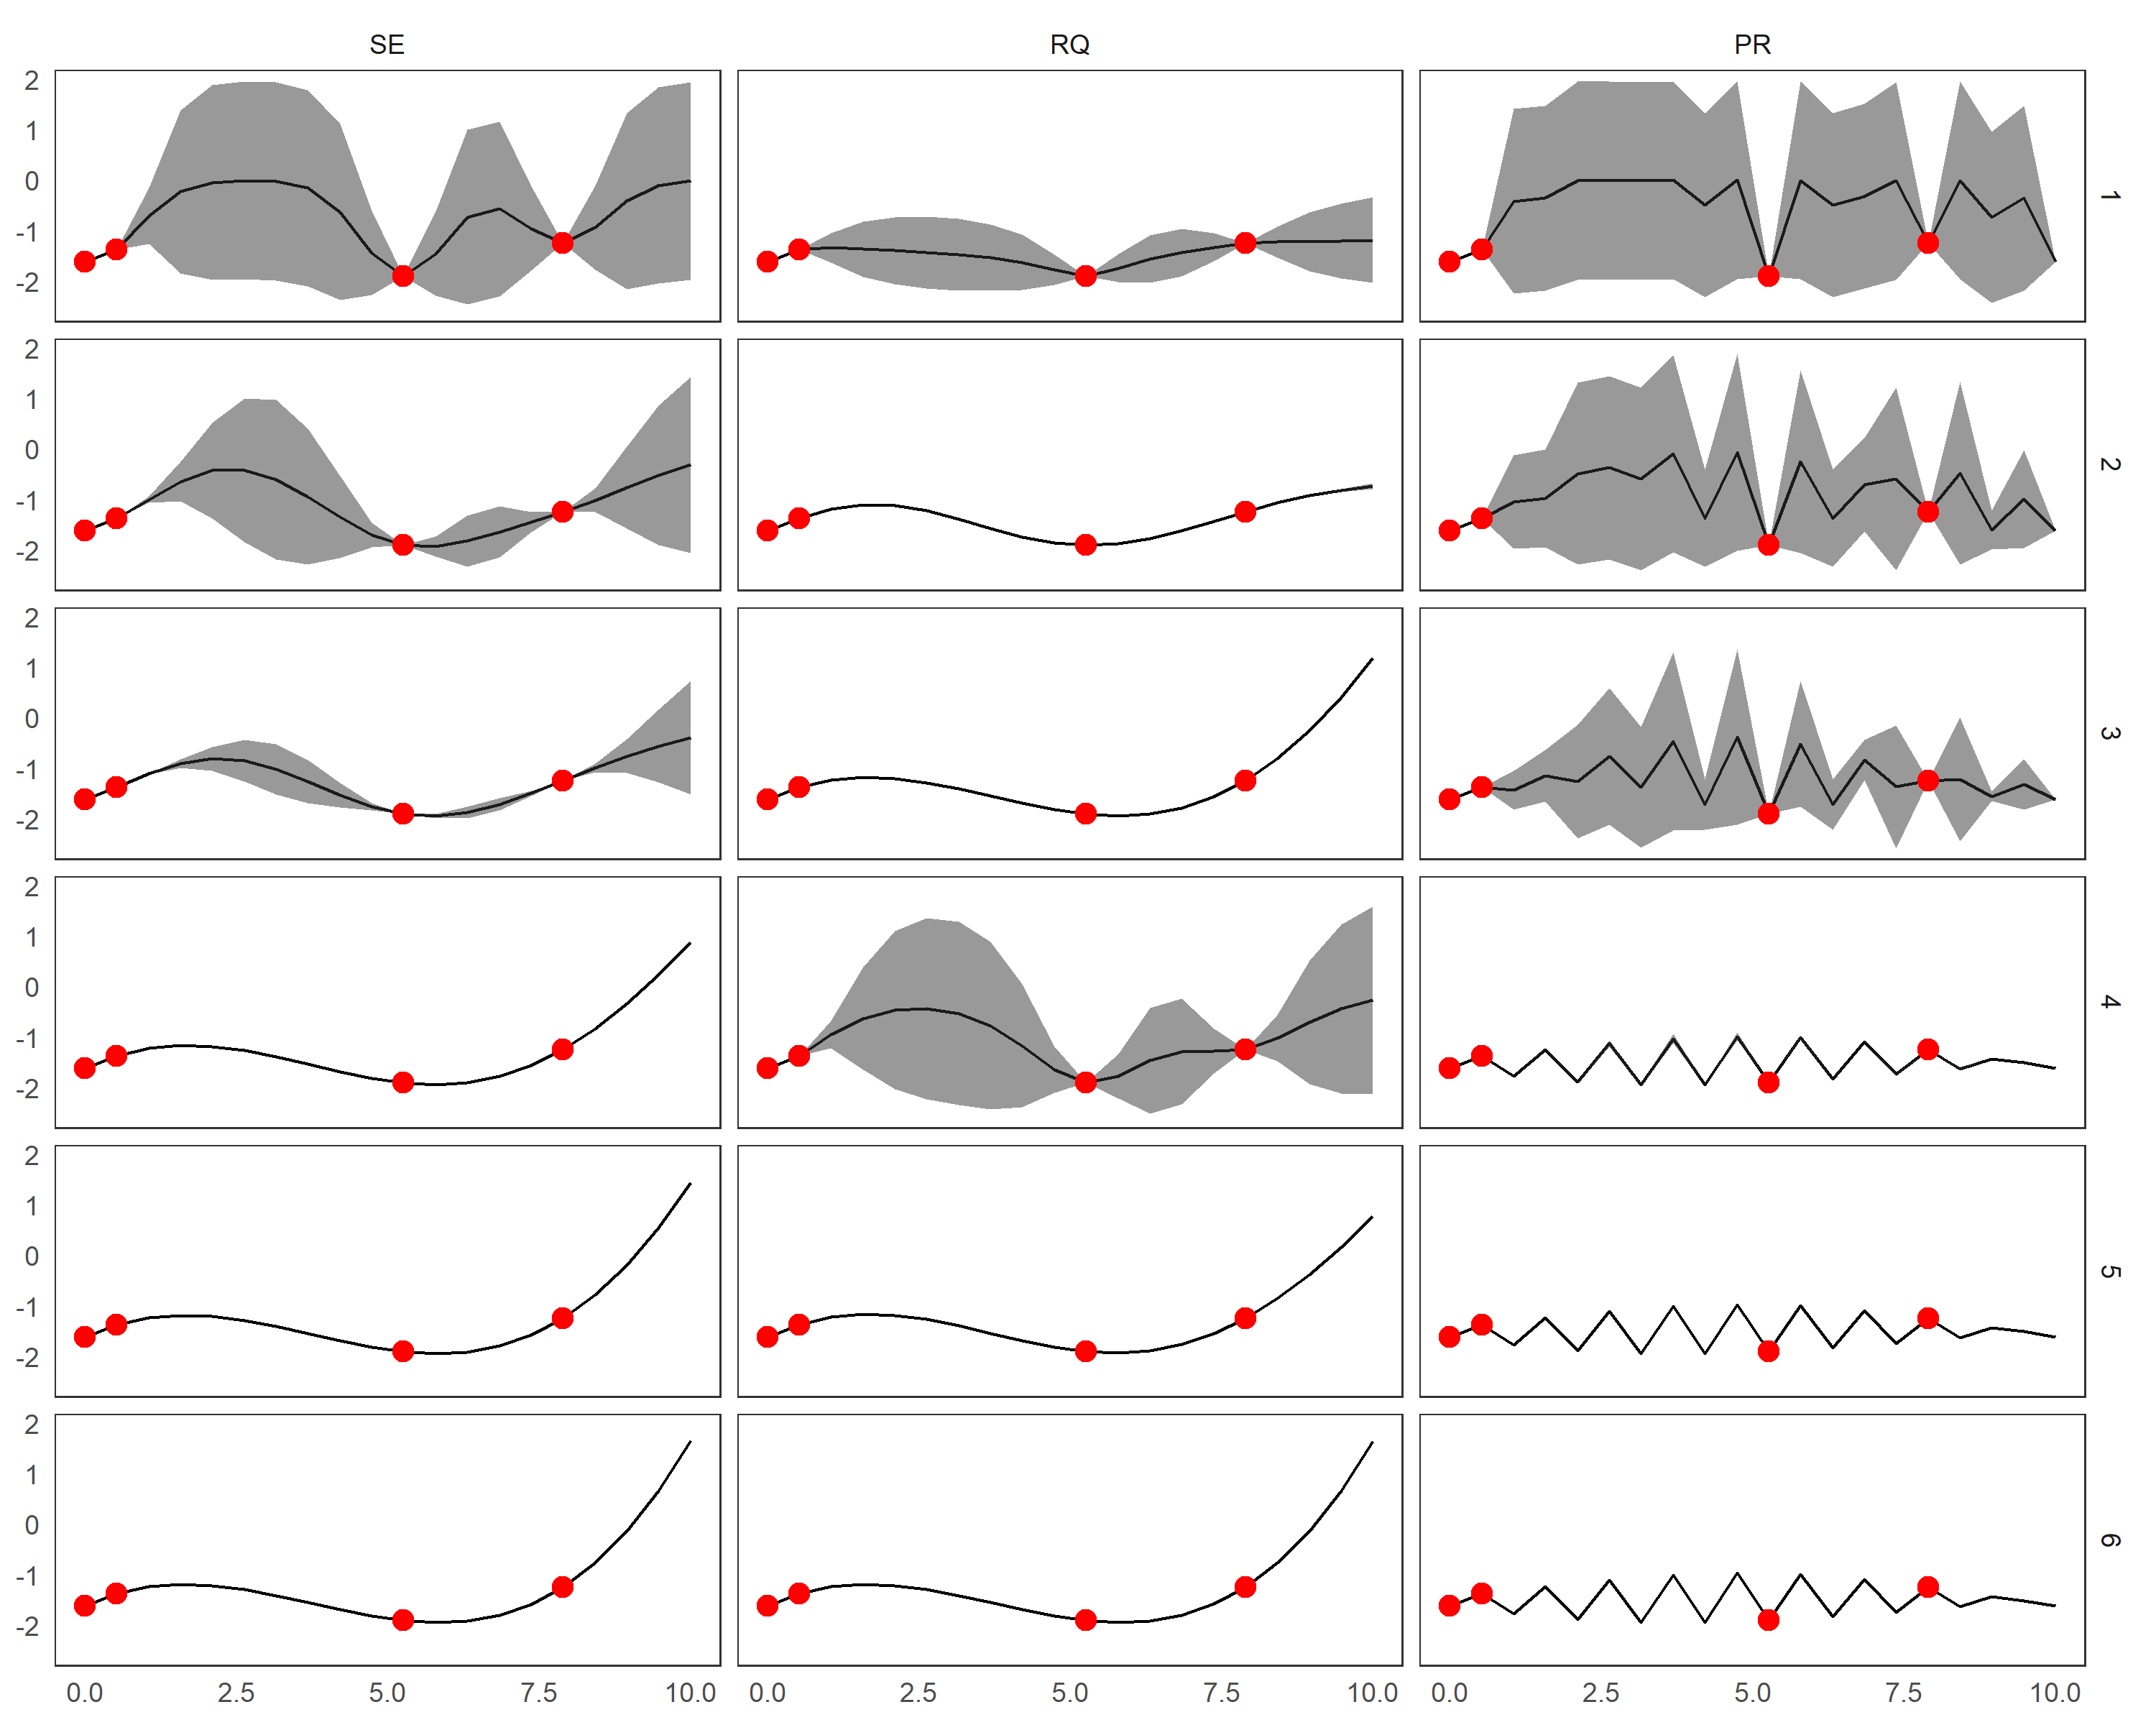
\includegraphics[scale = 0.15]{GP_illustrations/y_pred_stationary.png}
\caption{The predictive conditional mean of the IMF with the confidence intervals  under  noise-free assumption for different stationary kernel assumptions (columns wise) given 6 different sets of hyper-parameters. The red dots correspond to the observed values of the signal}\label{fig:}
\end{figure}



\paragraph{Non-stationary Kernels}
The non-stationary kernel can be characterised by a spectral density $\pi(\omega,\omega')$ such that
\begin{equation}
k(t,t') =\int \int \pi(\omega,\omega') e^{ 2 \pi i \omega t - \omega' t' }\ d\omega d\omega' = \mathbb{E}_{\omega,\omega'}\big[ \phi_{\omega,\omega'} (x) \phi_{\omega,\omega'} (x')^* \big] 
\end{equation}
where $\pi(\omega)$ is a spectral density of the kernel $k$ over frequencies $\omega$ and $\omega'$. For a scalar inputs $x$ and $x'$ the density $\pi(\omega,\omega')$ corresponds to bivariate distribution. 

\begin{enumerate}
\item Non-stationary generalisation of the Squared Exponential kernel (GSE)
\begin{align*}
k_{GSE}(t,t') = \sigma(t) \sigma(t') \bigg( \frac{2\mu(t) \mu(t')}{\mu(t)^2 +  \mu(t')^2}\bigg)^{-\frac{1}{2}} \exp \Big\{ - \frac{(t - t')^2}{\mu(t)^2 +  \mu(t')^2} \Big\} 
\end{align*}
for
\begin{align*}
& \log \sigma(t) \sim \mathcal{GP} \Big(\mu_\sigma, k_\sigma (t,t') \Big) \\
& \log \mu(t) \sim \mathcal{GP} \Big(\mu_\mu, k_\mu (t,t') \Big) \\
\end{align*}

\item Spectral Mixture Kernel by \citep{Remes2017}
% Non-Stationary Spectral Kernels, Remes 2017
which is formulated as follows
\begin{equation}
k_{SM}(t,t') = \sum_{q = 1}^Q w_q^2 \exp \Big\{ - 2 \pi^2 \tilde{\mathbf{t}}\bm{\Sigma}_q\tilde{\mathbf{t}}^T\Big\} \bm{\phi}_{\mu_q,\mu_q'} (t) \bm{\phi}_{\mu_q,\mu_q'} (t')
\end{equation}
where
\begin{align*}
\tilde{\mathbf{t}} = \begin{bmatrix}
t \\
- t'
\end{bmatrix} \text{ and } \bm{\phi}_{\mu_q,\mu_q'}(t) = \begin{bmatrix}
\cos (2 \pi \mu_{q} t) + \cos (2 \pi \mu_{q}' t)\\
\sin (2 \pi \mu_{q} t) + \sin (2 \pi \mu_{q}' t)
\end{bmatrix}.
\end{align*}
The spectral density of the kernel $k_{SM}$ is defined by a weighted mixture 
\begin{equation}
\pi(\omega,\omega') = \sum_{q = 1}^Q w_q^2 \pi_q(\omega,\omega)
\end{equation} 
where $\pi_q(\omega,\omega)$ is a sum of bivariate normal densities with two dimension mean vectors are equal to the the eight combinations of the two element permutations of the set $\big\{\mu_q,\mu_q'\big\}$ and $\big\{-\mu_q,-\mu_q',  \big\}$, and the covariance matrix $\bm{\Sigma}_q$.

\item Generalized Spectral Mixture Kernel by \citep{Remes2017} with Gibbs kernel formulations
% Non-Stationary Spectral Kernels, Remes 2017
which is formulated as follows
\begin{equation}
k_{GSM}(t,t') = \sum_{q = 1}^Q w_q(t) w_q(t') \bigg( \frac{2l_g(t) l_q(t')}{l_g(t)^2 +  l_q(t')^2}\bigg)^{-\frac{1}{2}} \exp \Big\{ - \frac{(t - t')^2}{l_q(t)^2 +  l_q(t')^2} \Big\} \cos \Big(2\pi (\mu_q(t) t - \mu_q(t') t') \Big) 
\end{equation}
for
\begin{align*}
& \log l_q(t) \sim \mathcal{GP} \Big(\mu_l, k_l (t,t') \Big) \\
& \log it \mu_q(t) \sim \mathcal{GP} \Big(\mu_\mu, k_\mu (t,t') \Big) \\
& \log w_q(t) \sim \mathcal{GP} \Big(\mu_w, k_w (t,t') \Big) 
\end{align*}

The spectral density of the kernel $k_{GSM}$ is ...



\item Sparse Spectrum Kernel by \citep{LazaroGredilla2010}
\end{enumerate}

